
\documentclass{standalone}
\usepackage[svgnames]{xcolor}
\usepackage{pgfplots}
\pgfplotsset{compat=newest}
\usepackage[sfdefault]{FiraSans}
\usepackage{FiraMono}
\renewcommand*\familydefault{\sfdefault}
\begin{document}
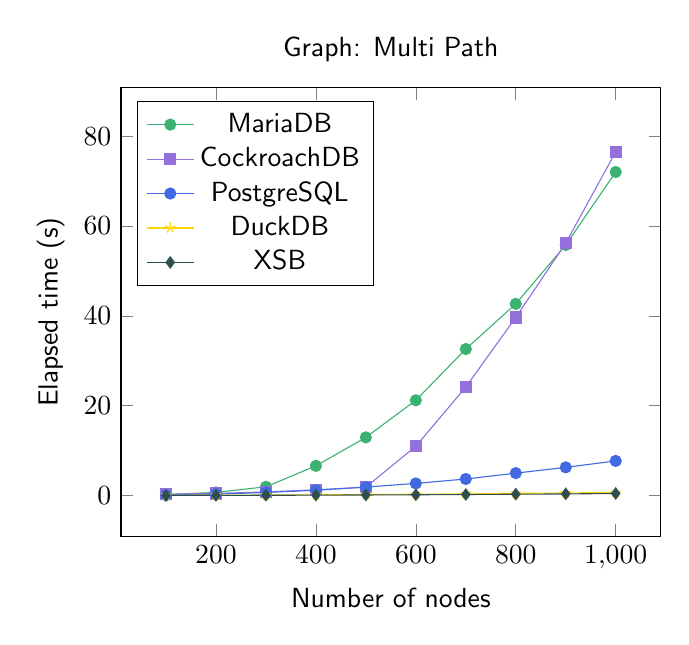
\begin{tikzpicture}
    \begin{axis}[
        title={Graph: Multi Path},
        xlabel={Number of nodes},
        ylabel={Elapsed time (s)},
        legend pos={north west},
        ymax=90.75665225982665
    ]
    \addplot+[MediumSeaGreen, mark options={color=MediumSeaGreen}] coordinates {(100,0.21733748358674349) (200,0.6737256000051275) (300,1.9297037998447195) (400,6.59034727497492) (500,12.930878700036555) (600,21.189158941409552) (700,32.60372614180669) (800,42.66726306662895) (900,55.780456374818456) (1000,72.01812755838037)};
\addlegendentry{MariaDB}
\addplot+[MediumPurple, mark options={color=MediumPurple}] coordinates {(100,0.2750395580078475) (200,0.4531949331983924) (300,0.7865893668029458) (400,1.2506771835964172) (500,1.8448262834106572) (600,10.965078658005222) (700,24.134830149798653) (800,39.63646629139548) (900,56.17867425840814) (1000,76.53208919160534)};
\addlegendentry{CockroachDB}
\addplot+[RoyalBlue, mark options={color=RoyalBlue}] coordinates {(100,0.05133122520055622) (200,0.29203119201119987) (300,0.6684507831931115) (400,1.1658416750025935) (500,1.8630006583873182) (600,2.682499316590838) (700,3.6655872417846695) (800,4.968861008400563) (900,6.256468641594983) (1000,7.688989308394957)};
\addlegendentry{PostgreSQL}
\addplot+[Gold, mark options={color=Gold}] coordinates {(100,0.021045975212473422) (200,0.04912799180019647) (300,0.09027067499700933) (400,0.13863869161577896) (500,0.1896437087794766) (600,0.2832283582072705) (700,0.34018262519966813) (800,0.46791438321815804) (900,0.5507885499973781) (1000,0.6813774999929592)};
\addlegendentry{DuckDB}
\addplot+[DarkSlateGray, mark options={color=DarkSlateGray}] coordinates {(100,0.004501152038574216) (200,0.017766809463500982) (300,0.039496564865112285) (400,0.0693380355834961) (500,0.1059611797332762) (600,0.1523663997650148) (700,0.21113691329956036) (800,0.2737027645111084) (900,0.3413739681243896) (1000,0.43467764854431146)};
\addlegendentry{XSB}

    \end{axis}
\end{tikzpicture}
\end{document}
